% Junior Level 1, Week 7 -- workbook chapter (read aloud by a grown-up)
\chapterweek{7}{Two Sprites Talk}{Each sprite has its own script; wait makes them take turns.}

\section{What you will learn}
\begin{ican}
  \item I can add a new sprite and a backdrop.
  \item I can make two sprites take turns to talk.
  \item I can say who made the pictures I use.
\end{ican}

\begin{exercise}[Hello, Ballerina!]
Make the cat and the Ballerina say hi.
\begin{enumerate}[leftmargin=1.4em,itemsep=2pt]
  \item Click \enquote{Choose a Sprite}. Pick the Ballerina.
  \item Click \enquote{Choose a Backdrop}. Pick one you like.
  \item Click the cat in the sprite list. Build the cat's script.
  \item Click the Ballerina. Build her script. She waits first.
  \item Click the green flag.
\end{enumerate}
\begin{center}
\begin{tabular}{c@{\qquad}c}
\textbf{Cat} & \textbf{Ballerina}\\[2pt]
\begin{scratch}[scale=0.8]
\blockinit{when \greenflag clicked}
\blocklook{say \ovalnum{Hi, Ballerina!} for \ovalnum{2} seconds}
\end{scratch}
&
\begin{scratch}[scale=0.8]
\blockinit{when \greenflag clicked}
\blockcontrol{wait \ovalnum{2} seconds}
\blocklook{say \ovalnum{Hi, Cat!} for \ovalnum{2} seconds}
\end{scratch}
\end{tabular}
\end{center}
\end{exercise}

\begin{exercise}[Boo at Once]
Omar's cat asks a question. The Ghost should answer after it. But they talk at the same time! Which sprite needs a wait? Draw an arrow to the spot.
\begin{center}
\begin{tabular}{c@{\qquad}c}
\textbf{Cat} & \textbf{Ghost}\\[2pt]
\begin{scratch}[scale=0.8]
\blockinit{when \greenflag clicked}
\blocklook{say \ovalnum{Who is there?} for \ovalnum{2} seconds}
\end{scratch}
&
\begin{scratch}[scale=0.8]
\blockinit{when \greenflag clicked}
\blocklook{say \ovalnum{Boo!} for \ovalnum{2} seconds}
\end{scratch}
\end{tabular}
\end{center}
Now build it on your Mac and fix it.
\end{exercise}

\begin{exercise}[My Two-Line Story]
Plan first. Pick two sprites. Draw who talks first and who answers. A grown-up can write the words.
\begin{center}
%% alt: Two big empty story boxes side by side for drawing. Box 1 is labeled first, with a speech bubble icon. Box 2 is labeled then, with a speech bubble icon and a small clock that means wait.
\begin{tikzpicture}[x=1cm,y=1cm]
  \draw[line width=1pt,rounded corners=4pt] (0,0) rectangle (7,4.5);
  \draw[line width=1pt,rounded corners=4pt] (7.6,0) rectangle (14.6,4.5);
  \node[anchor=north west,font=\bfseries] at (0.2,4.4) {1. First};
  \node[anchor=north west,font=\bfseries] at (7.8,4.4) {2. Then};
  \node[font=\Large] at (6.4,3.9) {\faComment[regular]};
  \node[font=\Large] at (13.15,3.9) {\faClock[regular]};
  \node[font=\Large] at (14.1,3.9) {\faComment[regular]};
\end{tikzpicture}
\end{center}
Now build it. Give the second sprite a wait.
\end{exercise}

\begin{grownup}[Giving credit]
Help your child say who made the pictures: \enquote{The sprites and backdrop were made by the Scratch team. The story is by me.}
\end{grownup}

\begin{vocab}
  \vocabword{backdrop}{The picture at the back of the stage.}
  \vocabword{credit}{Saying who made something, like a picture or a sound.}
\end{vocab}

\begin{reflection}
Draw your two sprites talking. How do you feel about your story? Circle one.

\begin{center}
\Huge\faSmile[regular]\qquad\faMeh[regular]\qquad\faFrown[regular]
\end{center}
\answerspace{3.5cm}
\end{reflection}
